\documentclass[tikz,border=10pt]{standalone}
% Shared look for every TikZ diagram. Load with % Shared look for every TikZ diagram. Load with % Shared look for every TikZ diagram. Load with \input{../../tools/tikz-style.tex}
\usepackage[T1]{fontenc}
\usepackage{lmodern}
\renewcommand{\sfdefault}{lmr}  % diagrams use the same serif as the text
\usetikzlibrary{arrows.meta, positioning, shapes.geometric, calc, fit, backgrounds}
\definecolor{cblue}{HTML}{4C78A8}
\definecolor{corange}{HTML}{F58518}
\definecolor{cgreen}{HTML}{54A24B}
\definecolor{cred}{HTML}{E45756}
\definecolor{cpurple}{HTML}{B279A2}
\definecolor{cgrey}{HTML}{6B6B6B}
\tikzset{
  every picture/.style={font=\sffamily, line width=1.2pt},
  box/.style={draw=#1, fill=#1!12, rounded corners=4pt, align=center, inner sep=7pt, minimum height=1.1cm},
  box/.default=cgrey,
  arrow/.style={-{Stealth[length=3mm]}, draw=cgrey, line width=1.4pt},
  title/.style={font=\sffamily\bfseries\Large},
  note/.style={font=\sffamily\small, text=cgrey, align=center},
}
\AtBeginDocument{\hyphenpenalty=10000 \exhyphenpenalty=10000}

\usepackage[T1]{fontenc}
\usepackage{lmodern}
\renewcommand{\sfdefault}{lmr}  % diagrams use the same serif as the text
\usetikzlibrary{arrows.meta, positioning, shapes.geometric, calc, fit, backgrounds}
\definecolor{cblue}{HTML}{4C78A8}
\definecolor{corange}{HTML}{F58518}
\definecolor{cgreen}{HTML}{54A24B}
\definecolor{cred}{HTML}{E45756}
\definecolor{cpurple}{HTML}{B279A2}
\definecolor{cgrey}{HTML}{6B6B6B}
\tikzset{
  every picture/.style={font=\sffamily, line width=1.2pt},
  box/.style={draw=#1, fill=#1!12, rounded corners=4pt, align=center, inner sep=7pt, minimum height=1.1cm},
  box/.default=cgrey,
  arrow/.style={-{Stealth[length=3mm]}, draw=cgrey, line width=1.4pt},
  title/.style={font=\sffamily\bfseries\Large},
  note/.style={font=\sffamily\small, text=cgrey, align=center},
}
\AtBeginDocument{\hyphenpenalty=10000 \exhyphenpenalty=10000}

\usepackage[T1]{fontenc}
\usepackage{lmodern}
\renewcommand{\sfdefault}{lmr}  % diagrams use the same serif as the text
\usetikzlibrary{arrows.meta, positioning, shapes.geometric, calc, fit, backgrounds}
\definecolor{cblue}{HTML}{4C78A8}
\definecolor{corange}{HTML}{F58518}
\definecolor{cgreen}{HTML}{54A24B}
\definecolor{cred}{HTML}{E45756}
\definecolor{cpurple}{HTML}{B279A2}
\definecolor{cgrey}{HTML}{6B6B6B}
\tikzset{
  every picture/.style={font=\sffamily, line width=1.2pt},
  box/.style={draw=#1, fill=#1!12, rounded corners=4pt, align=center, inner sep=7pt, minimum height=1.1cm},
  box/.default=cgrey,
  arrow/.style={-{Stealth[length=3mm]}, draw=cgrey, line width=1.4pt},
  title/.style={font=\sffamily\bfseries\Large},
  note/.style={font=\sffamily\small, text=cgrey, align=center},
}
\AtBeginDocument{\hyphenpenalty=10000 \exhyphenpenalty=10000}

\begin{document}
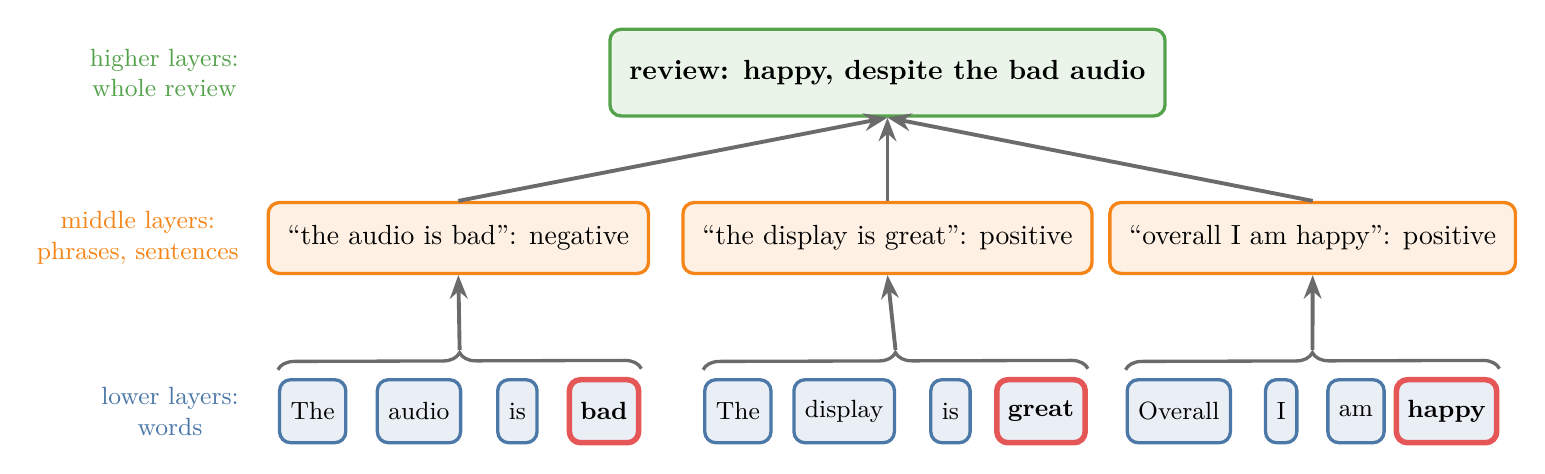
\begin{tikzpicture}[w/.style={box=cblue, inner sep=4pt, minimum height=0.8cm, font=\sffamily\small},
  k/.style={w, draw=cred, line width=2pt, font=\sffamily\small\bfseries},
  s/.style={box=corange, minimum height=0.9cm, font=\sffamily}, r/.style={box=cgreen, font=\sffamily\bfseries}]
  \foreach \t/\x/\st [count=\i] in {The/0/w, audio/1.35/w, is/2.6/w, bad/3.7/k, The/5.4/w, display/6.75/w, is/8.1/w, great/9.25/k, Overall/11.0/w, I/12.3/w, am/13.25/w, happy/14.4/k}
    \node[\st] (w\i) at (\x,0) {\t};
  \node[s] (s1) at (1.85,2.2) {``the audio is bad'': negative};
  \node[s] (s2) at (7.3,2.2) {``the display is great'': positive};
  \node[s] (s3) at (12.7,2.2) {``overall I am happy'': positive};
  \foreach \a/\b/\k in {1/4/1, 5/8/2, 9/12/3} {
    \draw[decorate, decoration={brace, amplitude=6pt}, cgrey] ([yshift=3pt]w\a.north west) -- ([yshift=3pt]w\b.north east);
    \draw[arrow] ($(w\a.north west)!0.5!(w\b.north east)+(0,0.35)$) -- (s\k.south);
  }
  \node[r] (rv) at (7.3,4.3) {review: happy, despite the bad audio};
  \foreach \k in {1,2,3} \draw[arrow] (s\k.north) -- (rv.south);
  \node[note, anchor=east, text=cblue] at (-0.8,0) {lower layers:\\words};
  \node[note, anchor=east, text=corange] at (-0.8,2.2) {middle layers:\\phrases, sentences};
  \node[note, anchor=east, text=cgreen] at (-0.8,4.3) {higher layers:\\whole review};
\end{tikzpicture}
\end{document}
